\graphicspath{{Chapter6/}}
\chapter{Intelligent Agents for Software Modeling Tasks}

The three empirical studies described in the previous chapters highlighted the strength of gamification as a motivator for student engagement, as well as an effective tool to support academic growth by increasing diagram quality and grades. The limitations tied to the two tool's evaluation systems, however, reduced their potential benefits, pointing to the need to find a way to extend the set of available solutions beyond the scope of synonyms and structures that can be identified by a single human. 

Additionally, the diffusion of large language models was becoming more and more common during the 2023-2024 academic year, showing several benefits and applications in the software engineering domain such as code generation and testing. Since the use of LLMs for model based engineering activities was still a relatively unexplored area in Autumn 2023, a new research direction was undertaken, with the goal of identifying ways in which intelligent agents could be used to support MBE activities such as diagram generation or evaluation.

For this purpose, two different research projects began in Autumn 2023, first as Master theses and then as complete studies, with the goal of observing an LLM's ability to generate valid diagram content, aiming to observe whether significant differences existed between the LLM-generated artifacts and student-produced diagrams: exploring this research area would provide insights on how agentic tools could be integrated in the teaching process and also derive guidelines for students on how to make better use of such tools. These two studies, focused respectively on UML class diagrams and UML use case diagrams were presented in \cite{debari2024evaluating} and \cite{garaccione2025vega}.

Following the results of these two studies, a third one was launched to implement a new software that could enhance the solution definition process for class diagrams by introducing LLM support: the architecture was created to be compatible with the Apollon library and create solution drafts starting from textual descriptions, both as editable diagrams and as data structures to be used with the evaluation engine. A preliminary proof of concept analysis was performed with two exercises, comparing the produced output diagrams with the reference solutions of existing exercises, identifying the limits of the architecture and allowing for the definition of next steps that guide the research activities to be performed after the end of the PhD. The new assistant was described in \cite{garaccione2026automated}.

Lastly, the findings from the first study led to subsequent theses that went beyond the original goal: instead of comparing human-made diagrams with those generated by a single architecture, new works were defined to compare multiple architectures on the same sets of requirements, with the goal of defining effective prompting strategies to enhance the solution-creating tool. One of these theses was then converted into a research article, and presented in \cite{garaccione2025models}.


%At the start of 2024 — the period in which the bulk of the empirical work in this chapter was initiated — the landscape of LLMs for SE was characterized by rapid capability growth but limited systematic evaluation on structured artifacts. The predominant models were GPT-4 (OpenAI) and Claude 2 (Anthropic), with emergent open-weight alternatives including Code Llama, Mistral, and early releases from Alibaba and DeepSeek. In the broader SE literature, reviews by Fan et al.~\cite{fan2023large} and Hou et al.~\cite{hou2023large} confirmed that diagram generation had received far less empirical attention than code-centric tasks, and the few available studies were limited to single-model evaluations with informal quality assessments.

%The research gap was particularly pronounced in the educational dimension. University-level SE courses routinely assign UML modeling exercises as formative and summative assessments. Instructors must create exercises, provide reference solutions, and evaluate student submissions — a workflow that is labor-intensive, especially at scale. Whether LLMs could produce solutions of sufficient quality to serve as reference examples, exercise templates, or automated grading aids was an open question with direct practical significance.

%This chapter reports four studies that address these gaps through a coherent research programme. The studies progress along two axes: the \textit{type of diagram} evaluated (class diagrams and use case diagrams), and the \textit{type of contribution} (empirical evaluation and tool construction). Taken together, they constitute a systematic exploration of LLM applicability for UML modeling in educational and tool-assisted contexts.


%\paragraph{Logical thread.} The four studies are connected by a progressive research logic. Study~1 poses the fundamental question of feasibility and establishes a quality baseline for class diagrams. Study~2 broadens the investigation to a second diagram type, probing the generalizability of the findings. Study~3 translates the empirical insights into a tool artefact that operationalizes LLM assistance in the educator's workflow. Study~4 revisits the evaluation with an improved methodology and a multi-model comparison, providing actionable guidance for practitioners and tool builders. Across all four studies, the educational frame is maintained: the stakeholder perspective is consistently that of the SE instructor or student, and the exercises are drawn from or modeled after real university curricula. This chapter thus documents a complete arc from initial feasibility assessment to comparative benchmarking and prototype tool realization.

%\paragraph{Relationship to the thesis.} The work in this chapter complements the preceding chapters of the thesis by addressing the AI-assisted dimension of the broader research programme on software modeling education. While Chapter~2 (UMLegend) investigated gamification as a pedagogical instrument for improving student engagement and diagram quality, this chapter investigates whether AI models can assist both sides of the educational transaction — providing reference solutions, exercise generation support, and potentially automated feedback. The two lines of inquiry converge on the goal of reducing the cost and improving the quality of SE education, with gamification acting on student motivation and LLMs acting on educator productivity and tool intelligence.



\section{Study 1: Evaluating Automatically Generated UML class diagrams}
%Study 1: Evaluating LLMs on UML Class Diagram Exercises

The first study started as a thesis in Autumn 2023, and had the goal of comparing an LLM's ability to generate class diagrams in comparison to a student. The goal for the study was to observe whether there were certain areas where an agent could perform similar to human solvers, or potentially even areas where it could outperform them. A controlled experiment was conducted using the data obtained with the thesis work to evaluate the LLM's ability against the human solver, with the design being formulated using the Goal-Question-Metric template according to Table  , expressing the goal as \textit{analyzing the use of LLM agents for the purpose of comparing the quality and correctness of generated UML Class Diagrams from natural language requirements, from the point of view of Software Modeling instructors}.

\begin{table}[ht]
\scriptsize
\centering
\caption{GQM Template for the study comparing LLMs and human solvers on UML class diagrams}
\label{tab_gqm}
    \begin{tabular}{ll}
    \toprule
    Object of study & Usage of LLM agents\\
    \midrule
    Purpose & Comparing artifacts\\
    Focus & Diagram quality, semantic correctness\\
    Context & Definition of UML Class Diagrams\\
    Stakeholders & Software Modeling Instructors\\
    \bottomrule
    \end{tabular}
\end{table}

\subsubsection{Study Design}
The first step to conduct the study was to collect exercises to compare LLM-generated and student-produced diagrams with; exercises were selected from various online sources, with the caveat that they had to provide a natural language description written in either English or Italian, and they had to be accompanied by a class diagram showing the intended reference solution. A total of 20 exercises were retrieved, covering several application domains and with a range of difficulties, allowing for multiple levels of comparison. 

Certain constraints were defined before conducting the study on both the student side and the LLM side, to ensure all exercises would be solved with the same conditions. For what concerns the student side, all 20 exercises were solved by the student for their thesis work with constraints set to simulate a real-life exam setting: a maximum of 30 minutes could be spent on solving each exercise, with neither any interaction with other people nor the use of any external sources such as textbooks, notes, or internet queries allowed. Diagrams were produced with the Microsoft Visio modeling tool-

Regarding the LLM, the model selected was OpenAI's ChatGPT-4, one of the best performing models at the time the study was conducted in Autumn 2023. No specific prompt engineering strategy was adopted, but rather, a simple prompt stating simply the goal and the format was employed:  

\begin{quote}
\textit{``Create a UML Class Diagram of the given exercise and give me the
PlantUML code''}, followed by the text of the exercise.
\end{quote}

The generated PlantUML code was then rendered graphically to generate image files, which were then used for the comparison with the corresponding student diagrams.

\subsection{Research Questions and Metrics}

The experiment was structured around two research questions:

\begin{itemize}
    \item[\textbf{RQ1:}] Does the use of LLM agents have an impact on the quality and correctness of UML Class Diagrams generated from natural language requirements?
    \item[\textbf{RQ2:}] What aspects of the natural language requirements have an impact on the quality of the generated UML Class Diagrams?
\end{itemize}

Diagram quality was measured according to the three dimensions identified by the framework by Bolloju and Leung \cite{bolloju2006assisting}, where, for each dimension, the total count of corresponding errors was computed. This meant identifying syntax errors such as the absence of multiplicity values or names in associations, the absence of attribute types, or the use of incorrect UML symbols, semantic errors such as incorrect values for a given association, the use of incorrect relationship types, incorrect attribute or method placement, or methods that could not be derived from relationships and attributes; lastly, pragmatic errors included redundant attributes or associations, specialization relationships with no way to distinguish subclasses, or style and layout inconsistencies in the graphical representation of the diagram. These three metrics can be computed through visual assessment of the diagrams, and syntax and pragmatic error counts can be computed without any comparison with reference solution, since they refer to intrinsic quality conditions that are applicable to any class diagram. 

A fourth metric used to answer RQ1 consisted of a \textit{correctness} measure equivalent to the semantic distance from each exercise's reference solution, computed using the method described by Nikiforova et al. \cite{nikiforova2015approach}: four separate distance vectors were computed for each dimension of the diagrams (classes and interfaces, attributes, methods, and relationships), leading to their aggregation into a single vector which was then used to calculate a scalar value equal to the distance between a given diagram and the reference solution; this value was then used to asses how close a diagram was to the reference, with lower distances identifying a more correct diagram and a distance of 0 identifying a semantically equivalent one.

RQ2, instead, focused on how certain aspects of the reference solutions and of the exercise descriptions could impact the solutions generated by the LLM: these aspects were the diagram \textit{Size}, computed as the sum of classes, attributes, methods, and associations in the reference solution, the \textit{Estimated difficulty} computed by three independent raters (three authors of the original article) and assessed before generating diagrams as the average of their rate expressed with a 1 (Easy to understand) to 5 (Hard to understand) Likert scale, and the \textit{Readability}, computed as the Flesch-Kincaid ease of readability score of the original description of each exercise \cite{solnyshkina2017flesch}. Reference measures were computed for the three metrics for each exercise, and are summarized in Table \ref{tab:ex_summary_llm4mod1}.


\begin{table}[ht]
\centering
\caption{Characteristics of the 20 exercises used in Study 1.}
\label{tab:ex_summary_llm4mod1}
\footnotesize
\begin{tabular}{cccccc}
\toprule
Exercise & Classes & Attributes \& Methods & Associations & Estimated Difficulty & Flesch-Kincaid score  \\
\midrule
1  & 6  & 17 & 7  & 2.33 & 45.9 \\
2  & 6  & 35 & 5  & 1.33 & 55.2 \\
3  & 7  & 12 & 8  & 4.67 & 67.5 \\
4  & 6  & 31 & 7  & 3.33 & 41.1 \\
5  & 8  & 18 & 11 & 2.33 & 48.4 \\
6  & 9  & 12 & 12 & 3.67 & 66.4 \\
7  & 6  & 5  & 7  & 1.00 & 58.6 \\
8  & 7  & 11 & 8  & 2.00 & 49.4 \\
9  & 9  & 13 & 10 & 2.67 & 54.7 \\
10 & 7  & 15 & 7  & 2.67 & 59.1 \\
11 & 6  & 11 & 9  & 3.33 & 55.4 \\
12 & 6  & 11 & 5  & 2.33 & 53.8 \\
13 & 8  & 19 & 8  & 1.67 & 58.0 \\
14 & 5  & 12 & 5  & 2.67 & 59.6 \\
15 & 8  & 6  & 8  & 4.33 & 74.5 \\
16 & 11 & 13 & 13 & 3.00 & 60.0 \\
17 & 8  & 5  & 8  & 2.33 & 53.1 \\
18 & 6  & 10 & 6  & 1.67 & 60.9 \\
19 & 9  & 20 & 9  & 4.00 & 54.5 \\
20 & 10 & 28 & 10 & 4.67 & 60.8 \\
\bottomrule
\end{tabular}
\end{table}


\subsection{Analysis Method}

Four null hypotheses were formalized to answer RQ1:

\begin{itemize}
    \item \textbf{${H_{0\_{syn}}}$:} The human or LLM-based generation of UML diagrams has no impact on the resulting syntactic quality;
    \item \textbf{${H_{0\_{sem}}}$:} The human or LLM-based generation of UML diagrams has no impact on the resulting semantic quality;
    \item \textbf{${H_{0\_{prag}}}$:} The human or LLM-based generation of UML diagrams has no impact on the resulting pragmatic quality;
    \item \textbf{${H_{0\_{corr}}}$:} The human or LLM-based generation of UML diagrams has no impact on the correctness of the diagram.
\end{itemize}

For each hypothesis, a one-way ANOVA test was applied, considering the solver type (either human or LLM) as the independent variable and each of the four RQ1 metrics (error counts for syntax, semantic, and pragmatic quality, semantic distance) as the dependent variable for the analysis. Bonferroni correction was applied to reduce the risk of Type-1 errors and have false positives, since four independent tests were conducted; as a consequence, the significance threshold was set to $\alpha_C = 0.05/4 = 0.0125$.

The analysis performed to answer RQ2, instead, relied on the results obtained with RQ1: in case significant differences among the quality metrics emerged from the statistical comparison, the goal was to observe whether size, readability, or difficulty had an influence on the affected quality dependent variable. It was decided to perform this analysis with a linear regression between all independent RQ2 variables and any resulting quality factor, with the main interest being the effect sizes rather than the p-values, given the low statistical power of the sample data; Bonferroni correction was applied in this case as well, however.


\subsection{Results}

Descriptive statistics for the four quality metrics associated with RQ1 are presented in Table \ref{tab:rq1_llm4mod1}: counts for syntax, semantic, and pragmatic errors, as well as semantic distance values, are grouped according to both the Human and LLM performance, and minimum, maximum, mean, median, and standard deviation are reported; the graphical distribution of the four metrics can be observed in

\begin{table}[ht]
\centering
\caption{Descriptive statistics for quality metrics in Study 1.}
\label{tab:rq1_llm4mod1}
\small
\begin{tabular}{lrrrrrrrr}
\toprule
& \multicolumn{4}{c}{Human} & \multicolumn{4}{c}{LLM} \\
\cmidrule(lr){2-5}\cmidrule(lr){6-9}
Metric & Min & Max & Mean (SD) & Median & Min & Max & Mean (SD) & Median \\
\midrule
Syntactic errors & 0 & 4  & 0.50 (1.14) & 0 & 0 & 2  & 0.90 (0.79) & 1 \\
Semantic errors  & 0 & 7  & 1.75 (1.80) & 1 & 0 & 14 & 4.85 (3.28) & 5 \\
Pragmatic errors & 0 & 4  & 1.10 (1.12) & 1 & 0 & 3  & 1.60 (0.94) & 1.5 \\
Distance         & 0.87 & 10.20 & 5.01 (2.36) & 4.24 & 2.24 & 11.54 & 7.25 (2.86) & 7.75 \\
\bottomrule
\end{tabular}
\end{table}


\begin{figure}[H]
    \centering
    \begin{subfigure}{0.5\linewidth}
        \centering
        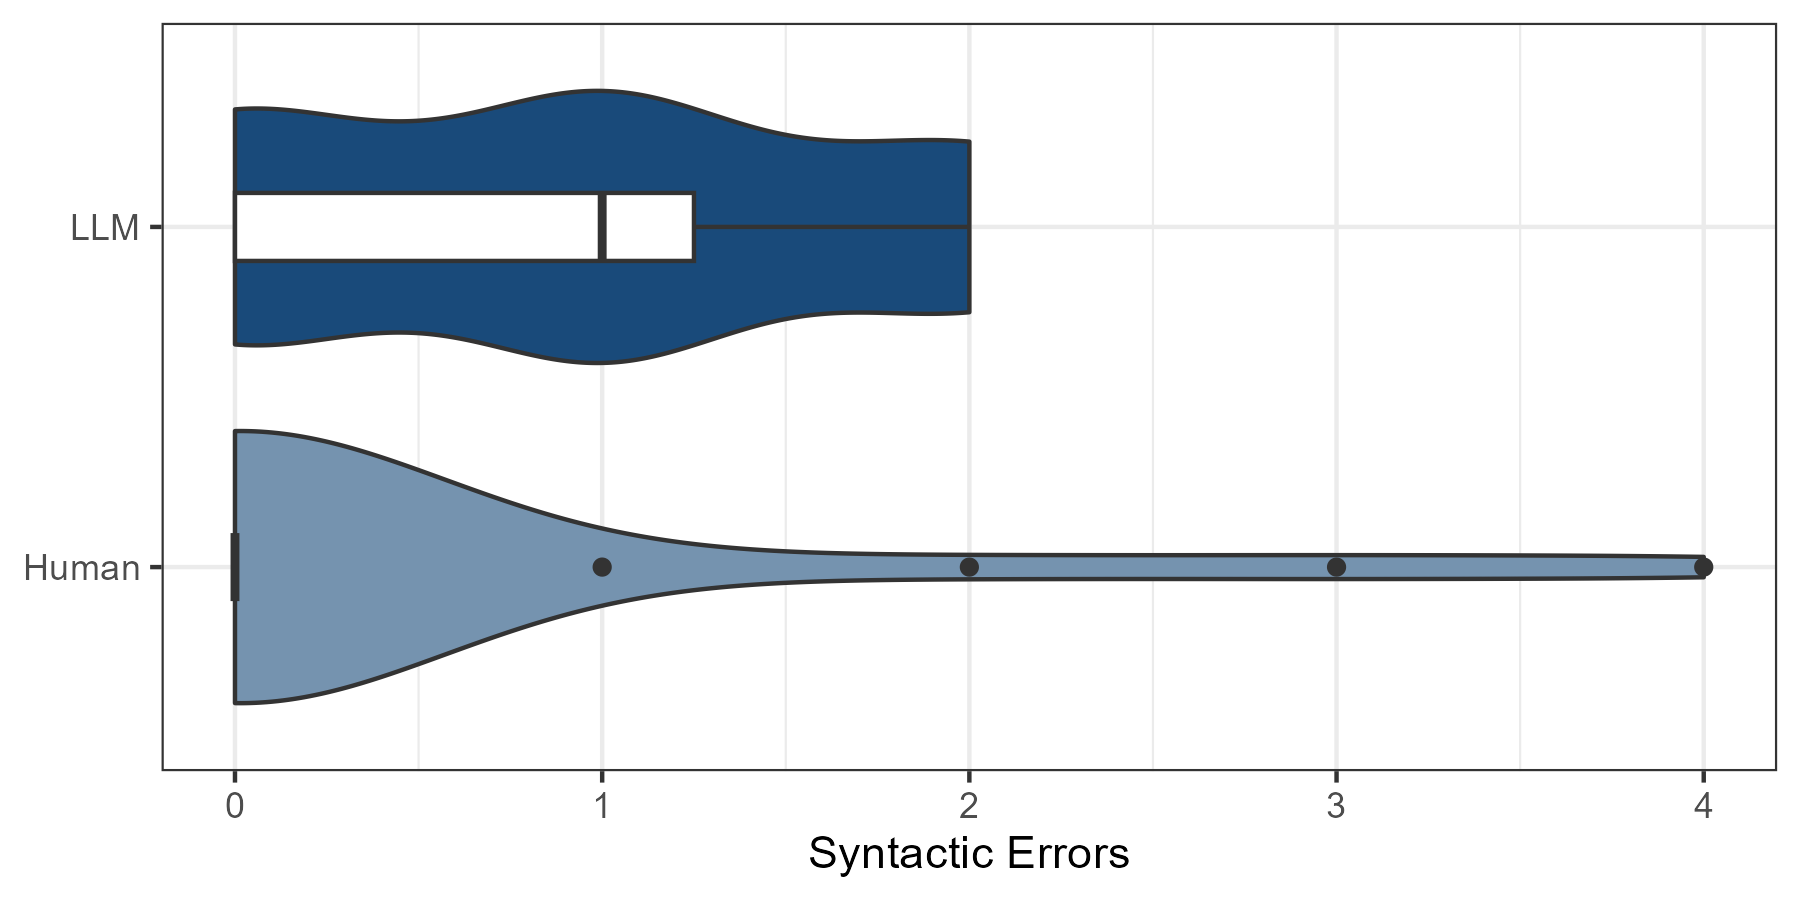
\includegraphics[width=\linewidth]{Template_Latex_ScuDo_Tesi/Chapter6/mod1_violin_syn.png}
        \caption{Box and violin plot for the count of \textit{Syntax Errors}}
        \label{fig:llm4mod1_syn}
    \end{subfigure}\hfill
    \begin{subfigure}{0.5\linewidth}
        \centering
        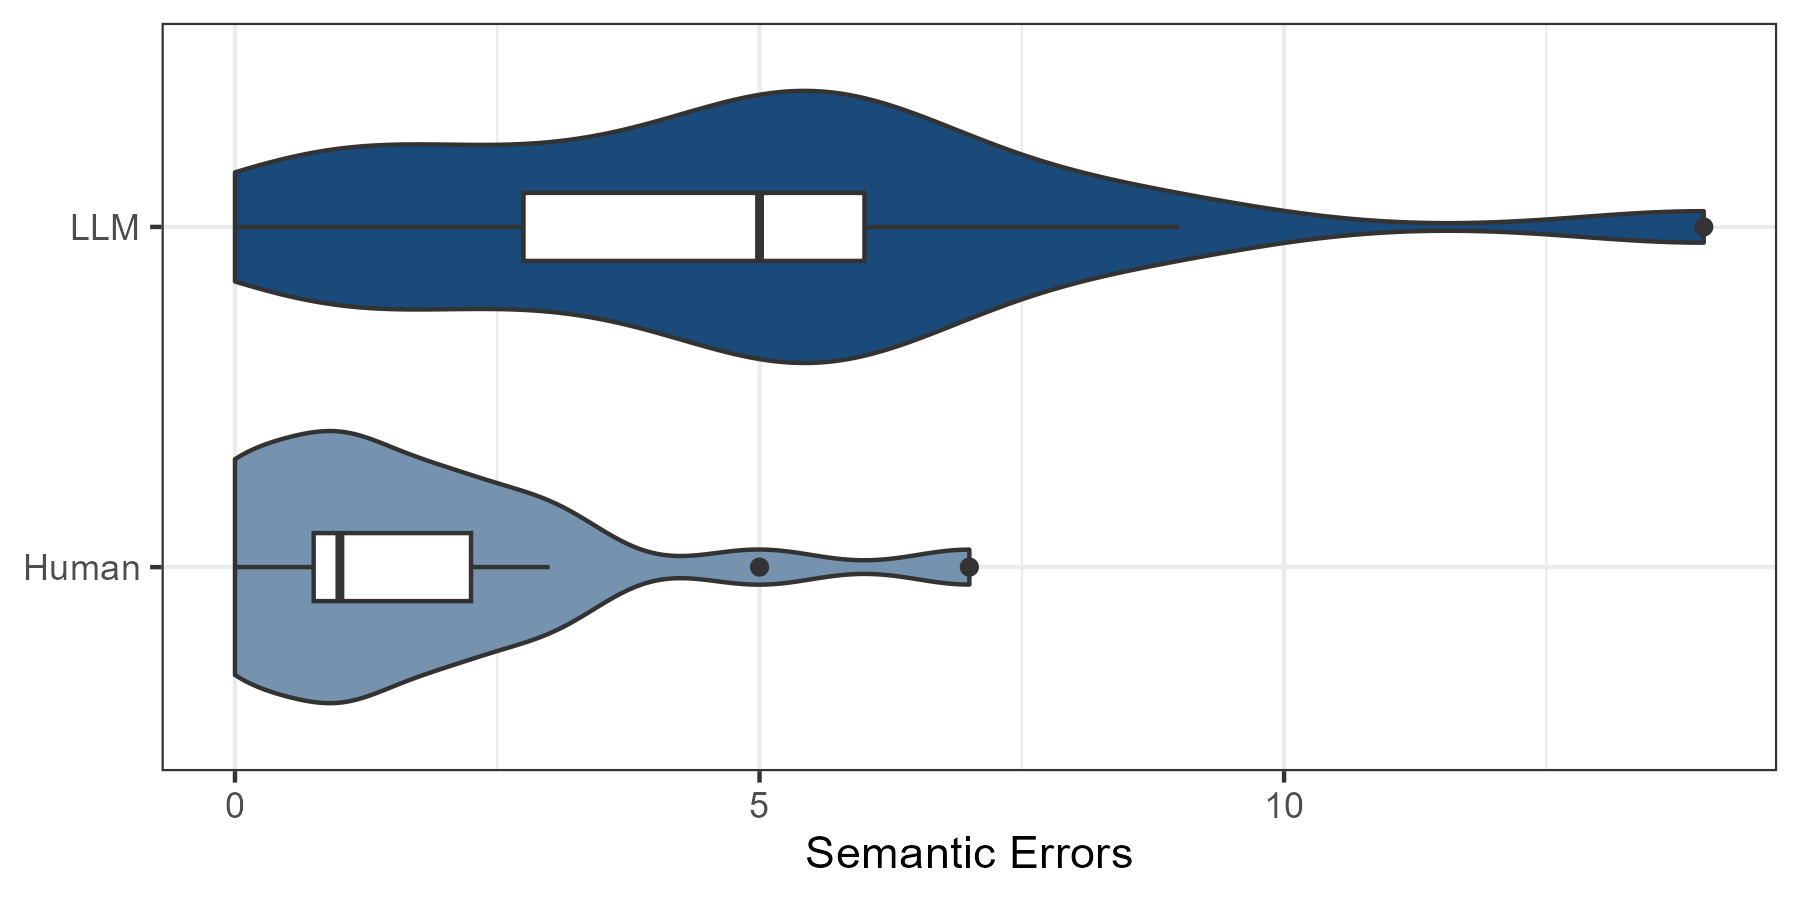
\includegraphics[width=\linewidth]{Template_Latex_ScuDo_Tesi/Chapter6/mod1_violin_sem.png}
        \caption{Box and violin plot for the count of \textit{Semantic Errors}}
        \label{fig:llm4mod1_sem}
    \end{subfigure}\hfill
    \begin{subfigure}{0.5\linewidth}
        \centering
        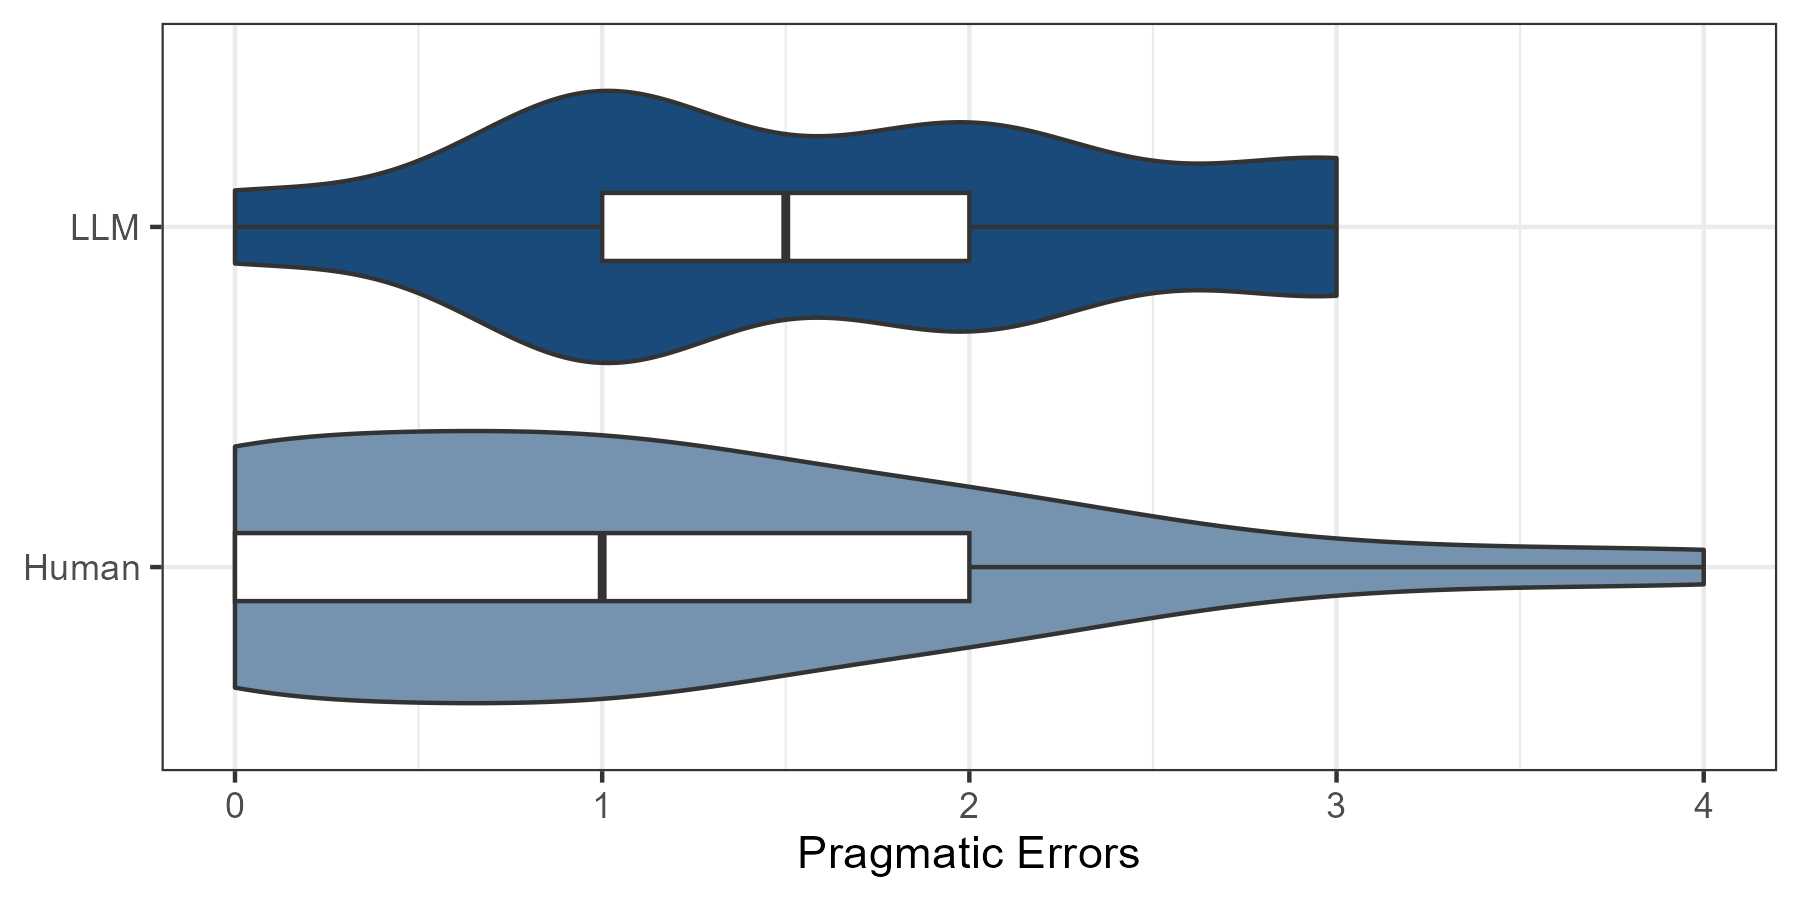
\includegraphics[width=\linewidth]{Template_Latex_ScuDo_Tesi/Chapter6/mod1_violin_prag.png}
        \caption{Box and violin plot for the count of \textit{Pragmatic Errors}}
        \label{fig:llm4mod1_prag}
    \end{subfigure}\hfill
    \begin{subfigure}{0.5\linewidth}
        \centering
        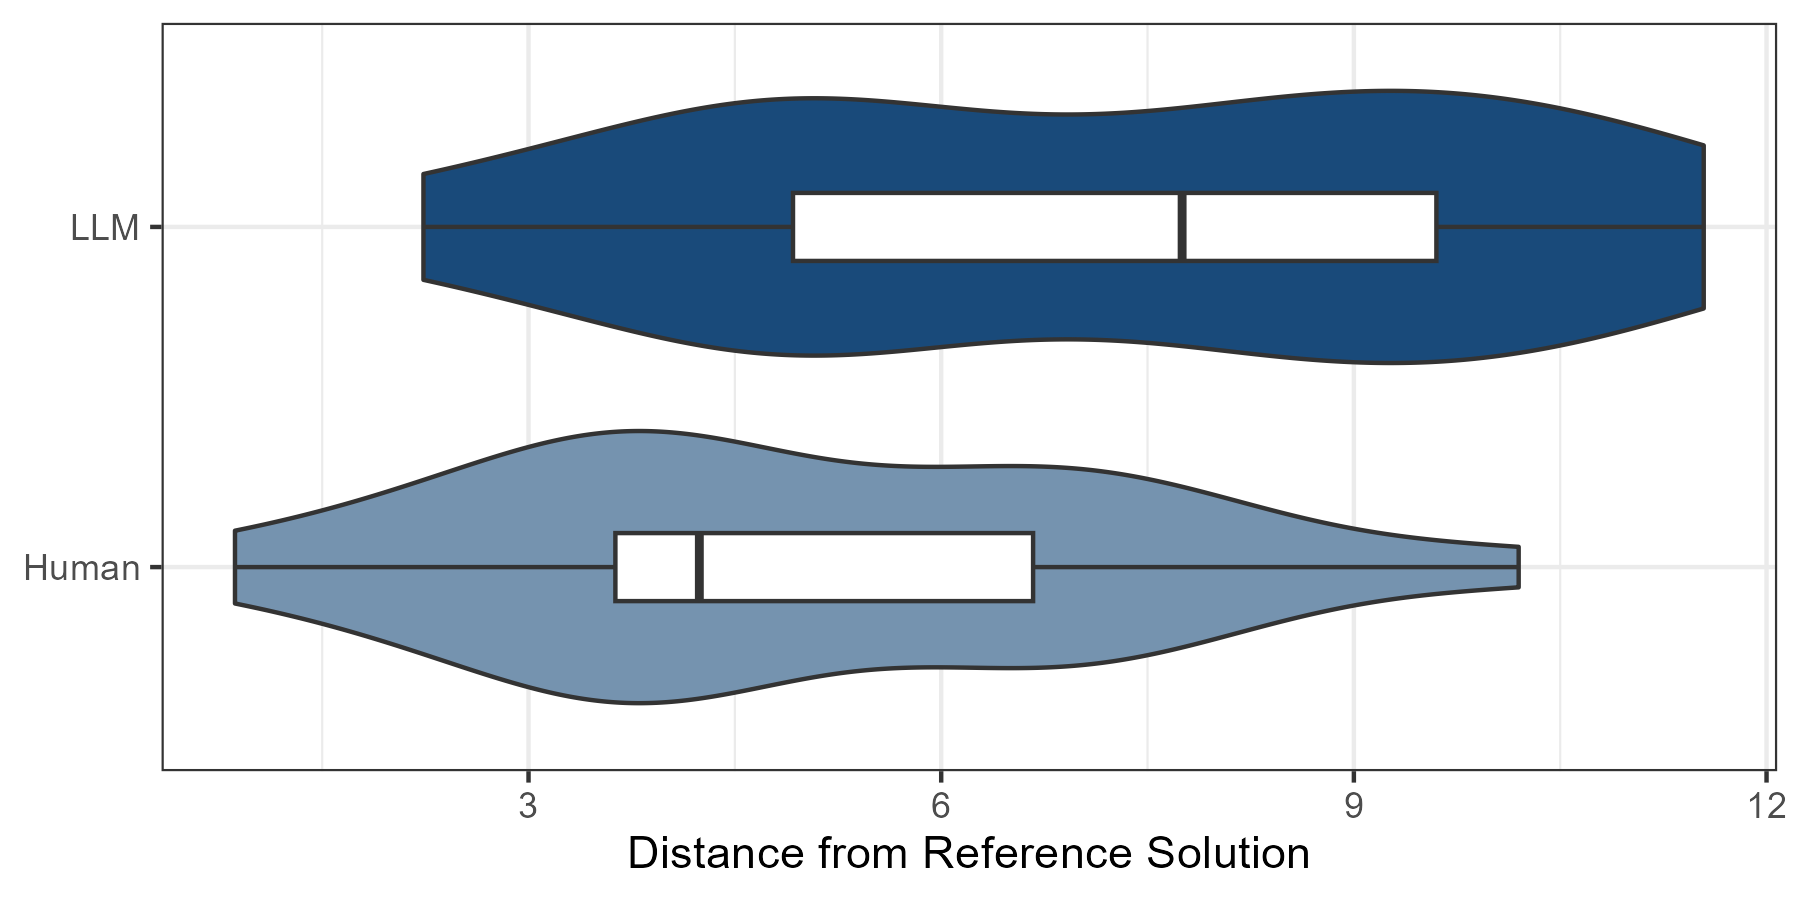
\includegraphics[width=\linewidth]{Template_Latex_ScuDo_Tesi/Chapter6/mod1_violin_dist.png}
        \caption{Box and violin plot for the \textit{Semantic Distance}}
        \label{fig:llm4mod1_dist}
    \end{subfigure}
    \caption{Box and violin plots for RQ1 metrics in the first study}
    \label{fig:rq2_4}
\end{figure}

Overall, it can be observed that the LLM agent performed worse compared to the human solver in all four metrics, with the highest difference being observed for the number of semantic errors, where ChatGPT obtained an average error count of 4.85, which is almost three times higher than the average count obtained by the student (1.75); maximum and median scores also accentuate this disparity, given a difference of 7 to 14 and 1 to 5, respectively. The reasonable assumption is that LLMs perform worse compared to humans when it comes to represent domain-specific details. The performance related to syntax and pragmatic errors is more balanced, however, with much lower differences in the average values for both counts. 

The ANOVA tests performed on the three error counts yielded a p-value of 0.206 for syntax errors, one of 6.7e-4 for the semantic count, and a p-value of 0.134 for pragmatic errors. The only statistically significant result is the second one: with the much lower average performance achieved by the LLM, the null hypothesis ${H_{0\_{sem}}}$ can be rejected, and it can be assumed that LLM agents are not yet able to produce class diagrams whose semantic quality is comparable to human-produced ones. The p-values related to the other two error metrics, instead, were not statistically significant, which means that ChatGPT can potentially display understanding of UML modeling rules and practices similar enough to those obtained by a student with sufficient knowledge.

Regarding semantic distance, the difference between the human solver and the LLM is once again prominent: the average distance is almost 50\% higher for the LLM agent and, in most exercises, the human solver managed to achieve a lower distance from the reference solution, suggesting a better ability to adequately represent the domain. Figure \ref{fig:llm4mod1_dum} plots the distances obtained by the two solvers across the 20 exercises: the LLM managed to outperform the student in two exercises and achieved the same distance in one. It is worth noting that these exercises exhibit a low number of elements in their reference solutions, although with variable estimated difficulty and readability scores: a low number of required elements may have been easier for the LLM to grasp and lead to more correct diagrams. 

\begin{figure}[ht]
    \centering
    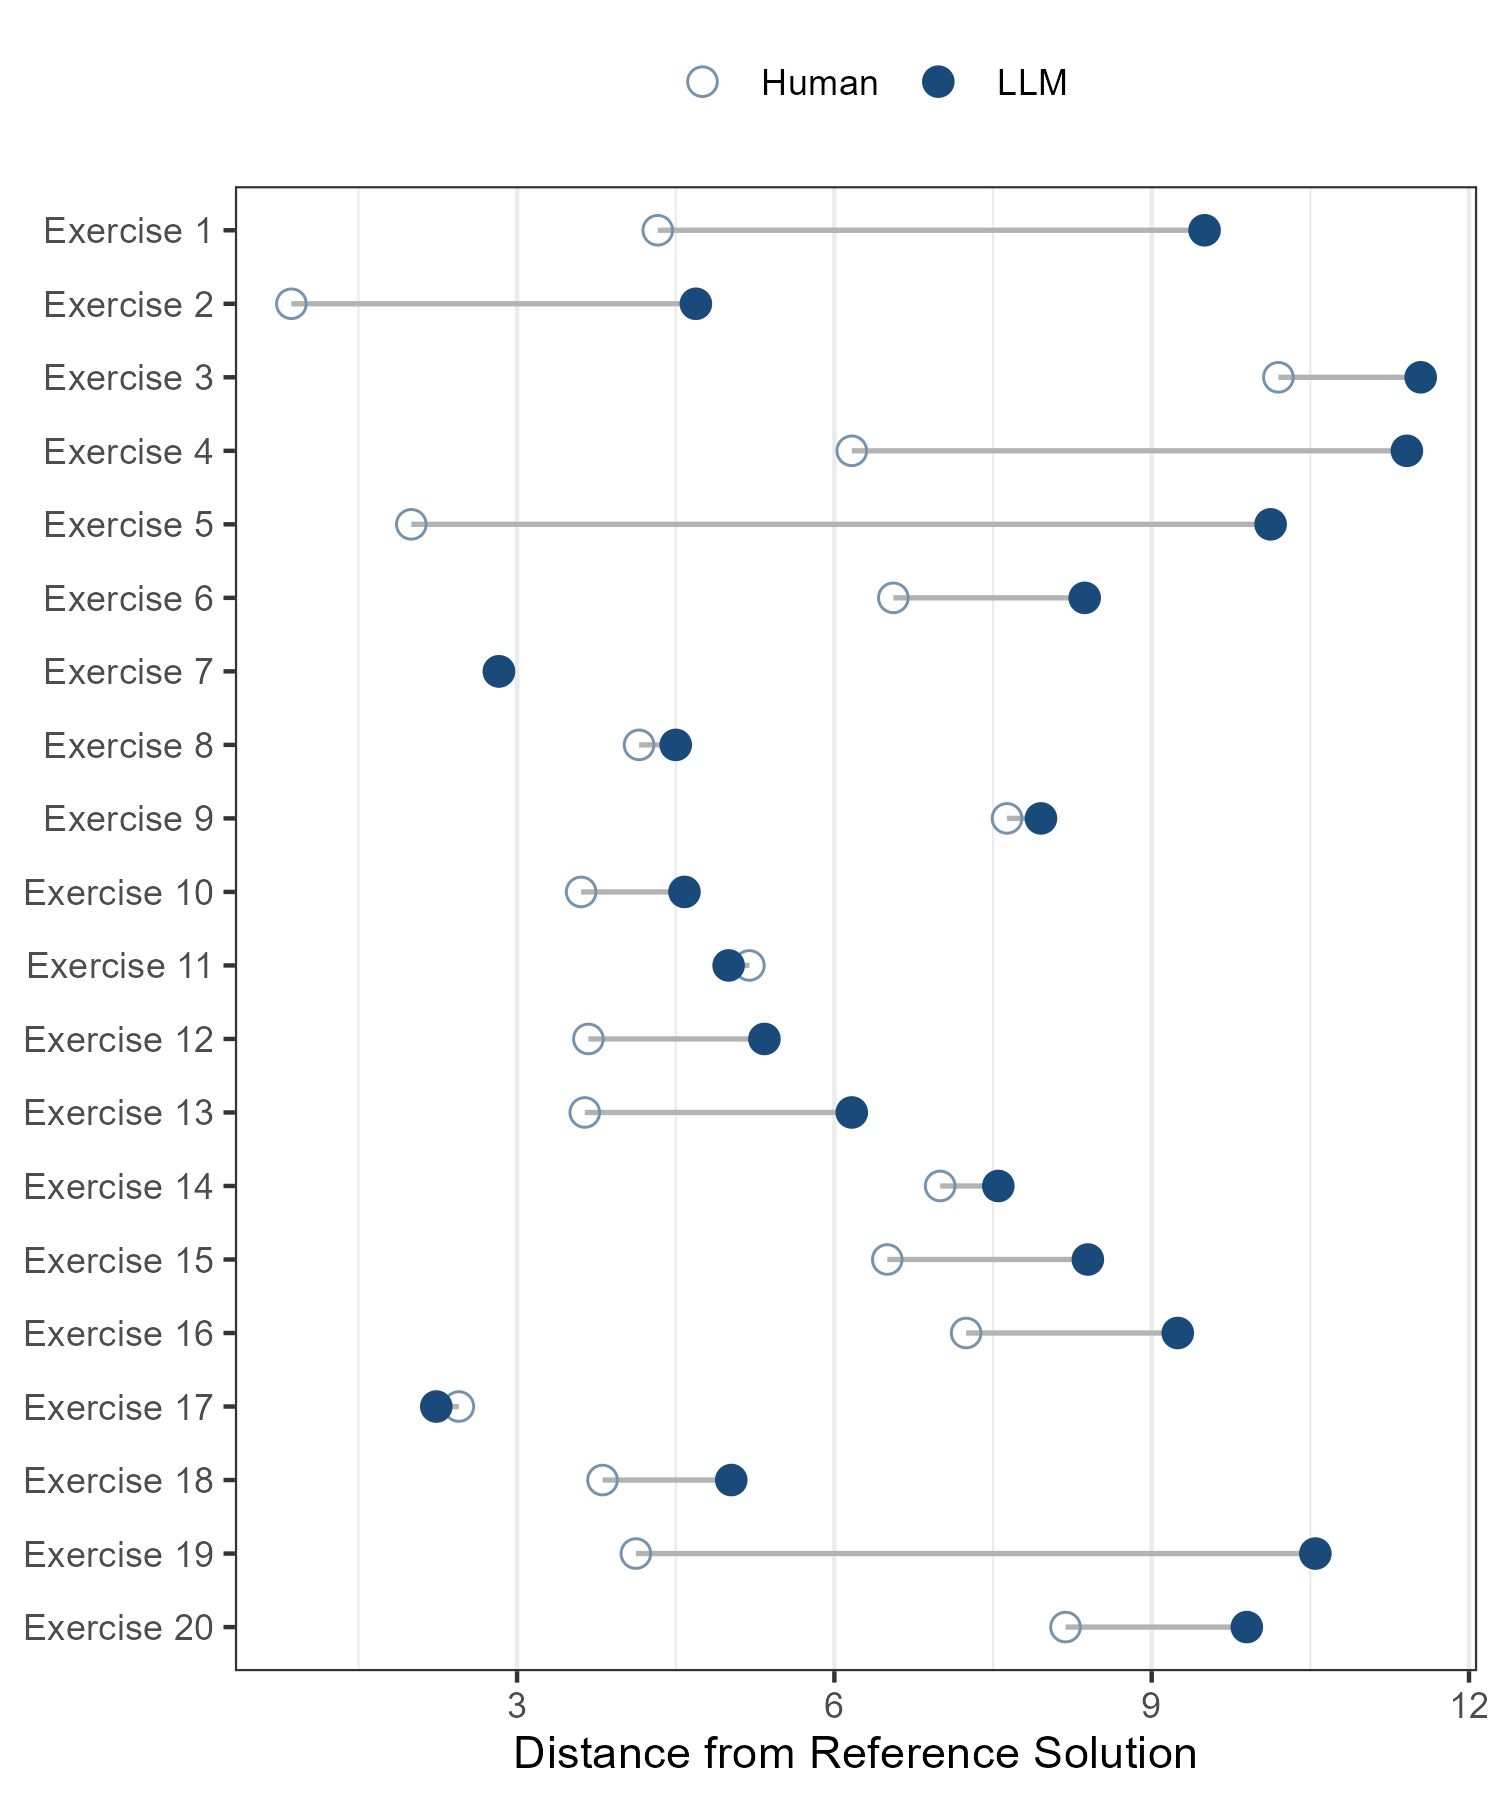
\includegraphics[width=0.75\linewidth]{Template_Latex_ScuDo_Tesi/Chapter6/mod1_dumbbell.png}
    \caption{Dumbbell plot showing the semantic distances obtained in the first study by the two solvers (Human vs. LLM)}
    \label{fig:llm4mod1_dum}
\end{figure}


The statistical test performed on the semantic distance obtained a p-value of 0.0102, which is lower than the Bonferroni-adjusted threshold: as a consequence, ${H_{0\_{corr}}}$ can be rejected, and it can be stated that LLMs perform worse when it comes to producing diagrams closer to an intended reference.

\answer{RQ1 (Study 1)}{The LLM solver performed significantly worse than the human in both semantic error count and semantic distance, showing a much lower ability to represent the details of the intended domains. The non-significant differences related to syntax and pragmatic quality indicate that, while still performing worse than a human expert, the agent presents a good understanding of UML modeling rules.}

The analysis identified statistically significant differences for what concerns the count of semantic errors and for the semantic correctness: these two metrics were thus selected as the dependent variables for RQ2, with the three size measures (classes, attributes+methods, associations), the estimated difficulty and the Flesch-Kincaid readability score as independent ones. However, before conducting the linear regression, a correlation matrix among the independent variables was defined, to assess whether there were some that needed to be removed due to depending among others; the correlation matrix is shown in Table \ref{tab:corrmatrix}.     

\begin{table}[ht]
\centering
\footnotesize
\caption{Correlation matrix of the independent variables for RQ2 in Study 1.}
\label{tab:corrmatrix}
\begin{tabular}{lccccc}
\toprule
                    & Classes & Attributes \& Methods & Associations & Estimated Difficulty & Flesch-Kincaid score \\
\midrule
Classes             & 1.000 & 0.034   & 0.851 & 0.439 & 0.270 \\
Attributes \& Methods &         & 1.000   & -0.080         & 0.073 & -0.397 \\
Associations &         &           & 1.000          & 0.411 & 0.151 \\
Estimated Difficulty &         &           &                  & 1.000 & 0.403 \\
Flesch-Kincaid score &         &           &                  &         & 1.000 \\
\bottomrule
\end{tabular}
\end{table}

Associations showed a high correlation level with classes, suggesting a strong linear association between them, leading to the exclusion of association from the set of independent variables used for the RQ2 analysis; the results of the linear regression are presented in Table \ref{tab:rq2_llm4mod1}, where, for each pair of independent and dependent variables, the estimate and the obtained p-value are reported. Given a total of 16 comparisons, the p-value threshold for significance was set as $\alpha_C = 0.003125$ following Bonferroni correction.

\begin{table}[ht]
\centering
\footnotesize
\caption{Linear regression results for RQ2 in Study 1 (significant p-values are in bold).}
\label{tab:rq2_llm4mod1}
\begin{tabular}{llllllllllllll}
    \toprule
        && Classes & ~ & ~ & Attributes \& Methods & ~ & ~ & Estimated Difficulty & ~ & ~ & Flesch-Kincaid score & ~ & ~ 
        \\
        ~ & ~ & estimate & SD & p-value & estimate & sd & p-value & estimate & sd & p-value & estimate & sd & p-value \\ \midrule
        Human & Semantic errors & 0.37 & 0.25 & 0.16 & -0.08 & 0.05 & 0.14 & 0.83 & 0.35 & 0.03 & 0.13 & 0.05 & 0.01 \\ 
        ~ & Distance & 0.49 & 0.33 & 0.15 & -0.03 & 0.058 & 0.72 & 1.67 & 0.34 & \textbf{1.0e-4} & 0.13 & 0.07 & 0.06 \\
        \midrule
        LLM & Semantic errors & 0.33 & 0.48 & 0.50 & 0.03 & 0.09 & 0.78 & 1.58 & 0.59 & 0.01 & 0.12 & 0.10 & 0.23 \\ 
        ~ & Distance & 0.63 & 0.39 & 0.13 & 0.13 & 0.08 & 0.08 & 1.84 & 0.46 & \textbf{8.1e-4} & -8.0e-4 & 0.09 & 0.99 \\ 
        \bottomrule
    \end{tabular}
\end{table}

The number of classes has a positive impact on both variables for both the human solver and the LLM: none of the coefficients are significant, however, implying that, while a higher number of classes can lead to an increased frequency of errors, both the student and the agent were able to correctly represent the main necessary elements in an UML exercise, even in cases with a high number of classes.

The sum of attributes and methods, instead, achieved a negative correlation with both dependent variables for the results obtained by the human solver: the interpretation is that, generally, humans tend to identify and derive attributes from natural language descriptions, making it easier to identify them and thus reducing the count of errors the more attributes are present in the reference solutions, which were in certain cases expressed in a minimal form, with only a subset of mandatory attributes among those that could be inferred from the descriptions.

The average estimated difficulty provided statistically significant p-values for the semantic distance for both the human solver and the LLM agent with positive estimates in both comparisons, implying that exercises that are recognized as more complex by domain experts are in fact harder to represent correctly; the slightly higher estimate for the LLM-generated exercises implies that agents struggle more with conventionally harder exercises. Lastly, the Flesch-Kincaid score had no significant impact on any variable: consequently, readability of the requirements cannot be stated as a proxy for modeling exercises' difficulty.


\answer{RQ2 (Study 1)}{The linear regression showed that classes had a positive effect on both metrics, albeit not significant, implying that diagrams with more necessary concepts are harder to represent for both solvers. Similarly, the estimated difficulty computed by expert evaluators led to significant increases in semantic distance for both solvers, showing that LLMs struggle for harder exercises similarly to how humans do.}


\subsection{Threats to validity.}

\textbf{Threats to internal validity:} the exercises selected for the study served as the correctness benchmark, and are thus the main cause of concern for the internal validity of the study. Solutions may be incomplete with regards to the original description, excessively detailed or simplistic, and consequently impact the computation of the semantic distances performed after the human assessment of the produced diagrams. Additionally, the somewhat limited prompt used for the LLM is also a threat, since other, more detailed prompts may have yielded better results and more correct diagrams; similarly, the unreliability of the LLM used for the study (ChatGPT-4) is another potential threat, since asking the same question to a different instance may lead to different results. Lastly, a single human solver performed all exercises, and said solver was the student who performed the original thesis work, introducing a bias in the exercises' correctness.

\textbf{Threats to external validity:} the sample of class diagram exercises was gathered from different educational sources, and the findings may not be generalizable to other types of modeling assignments. The selection of exercises aimed to cover multiple domains and include exercises with varying semantic content and difficulty level, to counteract this threat. The low sample size also limits the generalizability of the results.

\textbf{Threats to construct validity:} the produced solutions were evaluated following grading criteria and approaches widely adopted in research literature. It may however be possible to have used a different approach such as additional syntax and semantic grading rules, and, the methods used to assess diagrams are tailored for human solvers, they may not be suitable for LLM agents.

\textbf{Threats to conclusion validity:} the limited sample size of 20 exercises affects the ability to support the conclusions drawn from the study, and a more extensive set of exercises should be used to extend the study to assess whether the results obtained are actually consistent.


\subsection{Key findings}
\label{sec:llm4mde:study1:discussion}

The results show that an LLM, namely ChatGPT-4, with a single, unstructured, zero-shot prompt, can produce class diagrams that are structurally correct, readable, and understandable: the absence of significant differences for syntax and semantic errors shows that LLMs achieved a good understanding of class diagrams' formal grammar rules, leading to the creation of structurally valid diagrams.

However, a statistically significant worse performance for both semantic errors and distance shows that the model struggles to interpret and represent domain characteristics that may not be explicitly stated in the textual requirements. This dissonance between knowledge of syntax criteria and lack of semantic understanding suggests that LLMs struggle with domain-dependent constraints, and may not yet be effective for generating complete diagrams in educational context (e.g., examples of correct models, solutions for assignments), or even for industrial use during requirements definition or design specification.

Furthermore, the analysis on which of the exercise characteristics impacted quality metrics that showed significant differences showed that only estimated difficulty, derived from expert judgment, had a significant impact on quality, rather than the size of the reference solutions or the readability score of the textual requirements. The implication is that the cognitive challenge tied to modeling exercises is not tied exclusively to textual metrics but also requires domain intervention: as a consequence, integrating LLMs in model generation tasks should not rely exclusively on a description or a set of requirements, but additional guidance and annotation should be included to produce higher quality models.

\articleSummary{
color1
}{
Summary of Study 1
}{
The comparison of LLM-generated and student-produced class diagrams showed that intelligent agents achieve knowledge of syntax rules comparable to human solvers, but struggle more when it comes to semantic quality and ability to represent domain-specific requirements, with harder complexity affecting the produced diagrams' correctness. LLMs could be used to assist diagram generation but, without expert guidance and more complete prompts, the produced artifacts may only be used as preliminary drafts in educational contexts rather than complete solutions, since single-shot prompts struggle with more complex exercises and produce qualitatively valid diagrams only with simple sets of requirements.
}


\section{Study 2: Evaluating Automatically Generated UML use case diagrams}
%Study 2: Evaluating LLMs on UML Use Case Diagram Exercises
\subsubsection{Goal and Research Questions}

Building on Study~1, we designed a pilot study to assess LLM capability for
a structurally different diagram type — UML use case diagrams (UCDs). The
GQM goal is:

\begin{quote}
\textit{Analyze the use of LLM agents for the purpose of comparing UML Use
Case Diagrams generated from natural language requirements with human-made
ones, from the point of view of Software Modeling instructors.}
\end{quote}

\noindent The research questions are:

\begin{description}
  \item[RQ1] Does an LLM agent generate UML Use Case Diagrams whose
  \textit{completeness} differs from human-produced ones?
  \item[RQ2] Does an LLM agent generate UML Use Case Diagrams whose
  \textit{redundancy} differs from human-produced ones?
\end{description}

\subsubsection{Metrics}

\textbf{Completeness Rate} is defined as the ratio of correct elements in the
generated diagram to total elements in the reference solution. An element is
``correct'' if it matches a reference element in terms of name (or synonym) and,
for use cases, the associated actor. The metric ranges in $[0, 1]$.

\textbf{Redundancy Rate} is defined as the ratio of elements in the generated
diagram that do not match any reference element to the total number of elements
in the generated diagram. It ranges in $[0, 1]$; a value of 0 indicates no
superfluous elements.

Elements covered include actors, use cases, include relationships, and extend
relationships.

\subsection{Study Design}
\label{sec:llm4mde:study2:design}

\subsubsection{Exercise Collection}

Seventeen UCD exercises were collected from online Software Engineering
educational sources. Inclusion criteria: exercises in English, provided with
a reference solution. Reference solutions ranged from 6 to 17 elements (actors,
use cases, and relationships). Table~\ref{tab:study2:exercises} summarizes the
exercises.

\begin{table}[ht]
\centering
\caption{Summary of the 17 exercises in Study~2.}
\label{tab:study2:exercises}
\small
\begin{tabular}{rrrrr}
\toprule
Exercise & Actors & Use Cases & Includes & Extends \\
\midrule
1  & 4 & 7  & 0 & 0 \\
2  & 3 & 11 & 0 & 0 \\
3  & 4 & 8  & 0 & 0 \\
4  & 4 & 4  & 0 & 0 \\
5  & 2 & 7  & 3 & 0 \\
6  & 3 & 6  & 1 & 0 \\
7  & 1 & 5  & 0 & 0 \\
8  & 1 & 7  & 0 & 0 \\
9  & 6 & 7  & 0 & 0 \\
10 & 3 & 3  & 2 & 0 \\
11 & 4 & 7  & 1 & 3 \\
12 & 1 & 9  & 2 & 2 \\
13 & 5 & 11 & 0 & 1 \\
14 & 3 & 4  & 1 & 0 \\
15 & 2 & 7  & 0 & 0 \\
16 & 3 & 8  & 0 & 0 \\
17 & 2 & 12 & 0 & 0 \\
\bottomrule
\end{tabular}
\end{table}

\subsubsection{Human and LLM Solver Protocols}

The human solver protocol replicated the conditions of Study~1 (30-minute limit,
no external sources, individual work). Diagrams were produced using Signavio
Academic. The LLM was \textbf{ChatGPT-4}. The prompt was:

\begin{quote}
\textit{``The following should be textually analyzed, and a use case diagram
created containing several use cases. Identify the actors, use cases, and
associations. Please, use the user goal level approach. Also, please consider
any possible generalization relationship between use cases or between actors,
and any possible `include' or `extend' relationship between use cases.
Please give me the PlantUML code for the use case diagram corresponding to
the following text: (TEXT)''}
\end{quote}

Human and LLM solutions were evaluated by a second author (a software
engineering teacher) via comparison with reference solutions.

\subsubsection{Analysis Method}

A Wilcoxon signed-rank test was applied to answer both RQs, with solver type as
the independent variable. Bonferroni correction was applied for two tests:
$\alpha_C = 0.025$.

\subsection{Results}
\label{sec:llm4mde:study2:results}

Descriptive statistics are presented in Table~\ref{tab:study2:results}, and the
null hypotheses with $p$-values in Table~\ref{tab:study2:hypotheses}.

\begin{table}[ht]
\centering
\caption{Descriptive statistics for completeness and redundancy in Study~2.}
\label{tab:study2:results}
\small
\begin{tabular}{lrrrrrr}
\toprule
& \multicolumn{3}{c}{Human} & \multicolumn{3}{c}{LLM (ChatGPT-4)} \\
\cmidrule(lr){2-4}\cmidrule(lr){5-7}
Metric & Min & Max & Mean (SD) & Min & Max & Mean (SD) \\
\midrule
Completeness Rate & 0.29 & 1.00 & 0.82 (0.24) & 0.36 & 1.00 & 0.73 (0.23) \\
Redundancy Rate   & 0.00 & 0.50 & 0.17 (0.16) & 0.00 & 0.63 & 0.21 (0.21) \\
\bottomrule
\end{tabular}
\end{table}

\begin{table}[ht]
\centering
\caption{Null hypotheses and Wilcoxon test results for Study~2
($\alpha_C = 0.025$).}
\label{tab:study2:hypotheses}
\small
\begin{tabular}{llrp{2cm}}
\toprule
Hypothesis & Description & $p$-value & Outcome \\
\midrule
$H_{0,\text{compl}}$ & No impact on completeness rate  & 0.224 & Accept \\
$H_{0,\text{redun}}$ & No impact on redundancy rate    & 0.556 & Accept \\
\bottomrule
\end{tabular}
\end{table}

Neither completeness nor redundancy showed a statistically significant difference
between human and LLM solvers. While the LLM performed slightly worse on
average on both metrics (completeness 0.73 vs.\ 0.82; redundancy 0.21 vs.\
0.17), these differences are not statistically distinguishable given the sample
size. The human solver achieved optimal completeness (rate = 1.0) on 8 exercises,
and the LLM on 4; the human achieved zero redundancy on 4 exercises, as did
the LLM. No LLM solution simultaneously achieved optimal completeness and zero
redundancy, while the human achieved this in two cases.

\subsection{Discussion}
\label{sec:llm4mde:study2:discussion}

The results of Study~2 contrast with those of Study~1 in an instructive way: for
use case diagrams, LLM and human performance are statistically comparable across
completeness and redundancy, whereas for class diagrams (Study~1), the LLM
exhibited significantly worse semantic quality. This divergence is interpretable
in terms of the structural differences between the two diagram types.

Use case diagrams capture functional requirements at a relatively high level of
abstraction: they identify actors and named goals without requiring cardinality
constraints, type annotations, or complex relationship semantics. Class diagrams,
by contrast, require precise cardinality labels, correct distinction between
association types, and accurate placement of attributes and methods — all of
which are domain-specific semantic choices that go beyond the surface patterns
present in typical LLM training corpora. The simpler semantic requirements of
use case modeling appear to be better aligned with LLM capabilities in natural
language understanding and goal identification.

The observation that LLMs tend to include superfluous elements (higher maximum
redundancy rate of 0.63 vs.\ 0.50) suggests a tendency toward
\textit{over-generation}: the model includes actors or use cases that are
plausibly related to the described system but are not part of the expected
solution. This is consistent with the known hallucination tendency of LLMs and
with the semantic error pattern observed in Study~1.

The findings support the use of LLM agents for first-pass use case modeling
assistance, with the expectation that human review will be needed to prune
redundant elements and verify completeness. As with Study~1, the one-shot nature
of the prompt leaves substantial room for improvement through iterative refinement
or multi-turn dialogue strategies.

\paragraph{Threats to validity.}
\textit{Internal validity} threats include the use of a single human and a single
LLM solver, and the inherent limitations of reference solutions as ground truth.
\textit{External validity} is limited by the 17-exercise sample.
\textit{Construct validity} is threatened by the completeness and redundancy
metrics, which do not capture all quality dimensions of use case diagrams.
\textit{Conclusion validity} is limited by the small sample size.


\section{Development of an assistant for the creation of modeling exercises solutions}
%Study 3: TIGRE — A Tool for LLM-Assisted Reference Solution Generation
Studies~1 and 2 evaluated LLM capability in a purely assessment-oriented frame.
Study~3 translates these empirical insights into a tool contribution. The
motivation derives from three observations from the preceding studies: (a)~LLMs
can produce structurally plausible diagrams that capture most relevant domain
concepts; (b)~LLM outputs consistently require human correction in semantic
details; (c)~the workflow of LLM-based generation followed by human correction
is only tractable if the LLM output is rendered in a directly editable form
rather than as text or PlantUML code.

The objective of Study~3 is therefore to design, implement, and conduct a
proof-of-concept validation of \textbf{TIGRE} (auTomated dIagram Generator of
REference solutions), a web-based platform that integrates LLM-assisted diagram
generation with a visual modeling canvas and a structured reference data model
for educational use.

\subsection{Study Design}
\label{sec:llm4mde:study3:design}

\subsubsection{Tool Architecture}

TIGRE is implemented as a React-based web application. Its core modeling
component is \textbf{Apollon}~\cite{apollon}, an open-source web-based UML
editor that supports class diagrams and renders them as interactive canvas
elements. LLM integration is realized via HuggingFace's API services. For this
proof of concept, \textbf{DeepSeek R1-Distill-Qwen-32B} was selected as the
LLM backend due to its strong reasoning performance and open-source availability.

The tool supports two types of reference data objects for each exercise:

\begin{description}
  \item[Model object] A diagram representation compatible with the Apollon
  editor, listing classes (with attributes, methods, and graphical layout
  metadata) and relationships (with type, connected classes, cardinality, and
  graphical details). Models can be drawn interactively on the canvas or
  generated from LLM output.
  \item[Structure object] A notation-independent specification of the required
  elements for an exercise, used as the basis for automated evaluation. It
  contains: a list of required classes (with synonyms, weights, forbidden
  attributes, and expected attributes); a list of required associations (with
  allowed multiplicities); a list of required enumerations; and constraint lists
  (class names that are forbidden, pairs of classes that must not be directly
  associated).
\end{description}

The LLM-assisted workflow operates as follows. A teacher provides the exercise
text to DeepSeek, which returns the expected set of elements. The response is
parsed and converted into both a model object (rendered immediately on the
canvas) and a structure object (populated in the editing form). The teacher can
then edit both representations. Additionally, the LLM can be invoked to generate
synonyms for named elements in the structure, broadening the accepted solution
space for automated evaluation.

TIGRE supports the definition of multiple alternative reference solutions for a
single exercise, further extending the coverage of valid solution variants.

\subsubsection{Proof-of-Concept Evaluation}

To assess the initial capabilities of TIGRE, two class diagram exercises were
selected from past exams of the Information Systems course at Politecnico di
Torino. The exercises are labelled \textsc{Hackathons} and \textsc{Ski Passes}.
TIGRE was used to generate reference solutions for both, which were then
compared with teacher-defined reference solutions using the semantic distance
method of Nikiforova et al.~\cite{nikiforova2015approach}.

The evaluation procedure was: (i)~match each reference class to the most
semantically similar generated class, with unmatched classes scored 1;
(ii)~match attributes within matched class pairs by name and type;
(iii)~match associations if both connected classes are matched and the
association type and cardinality are equal; (iv)~compute individual distance
scores for classes, attributes, and associations, then aggregate into an overall
diagram distance. The procedure was performed by one author and reviewed by
the other two authors independently.

\subsection{Results}
\label{sec:llm4mde:study3:results}

Table~\ref{tab:study3:results} reports the element counts and distance scores
for both exercises.

\begin{table}[ht]
\centering
\caption{Summary evaluation metrics for the two exercises in Study~3.}
\label{tab:study3:results}
\begin{tabular}{lrr}
\toprule
Metric & \textsc{Hackathons} & \textsc{Ski Passes} \\
\midrule
Reference classes        & 10 & 7  \\
Reference attributes     & 19 & 26 \\
Reference associations   & 14 & 6  \\
Generated classes        &  9 & 9  \\
Generated attributes     & 10 & 22 \\
Generated associations   &  8 & 8  \\
\midrule
Class distance           & 2.40 & 2.96 \\
Attribute distance       & 4.58 & 5.83 \\
Association distance     & 3.87 & 3.16 \\
Diagram distance         & 6.46 & 7.26 \\
\bottomrule
\end{tabular}
\end{table}

Class distance scores were relatively low in both exercises, indicating
reasonable class identification. In \textsc{Hackathons}, 7 of 10 reference
classes were matched, though 3 had naming mismatches and 2 were unnecessary.
In \textsc{Ski Passes}, only 4 of 7 reference classes were matched, with 5
unnecessary generated classes (replacing attributes or representing irrelevant
concepts).

Attributes showed the highest distance scores in both exercises. In
\textsc{Hackathons}, 7 of 19 reference attributes were matched (only 2 exactly
by name and type); in \textsc{Ski Passes}, 9 of 26 were matched (2 attributes
and 3 enumeration literals exactly).

Associations showed moderate distance scores. In \textsc{Hackathons}, 6 of 14
reference associations were matched by name but only 1 had a correct cardinality;
in \textsc{Ski Passes}, all 3 matched associations had incorrect 1-1
cardinalities, reflecting a systematic failure to capture many-to-many and
one-to-many relationships.

\subsection{Discussion}
\label{sec:llm4mde:study3:discussion}

The proof-of-concept results confirm the findings of Study~1 in a tool-mediated
setting: LLMs can identify the core classes of a domain model but consistently
introduce errors in cardinality specification and include unnecessary elements.
The key contribution of TIGRE with respect to prior work is not the diagram
generation capability per se, but the \textit{tooling infrastructure} around it:
LLM output is automatically converted into an editable diagram on a visual
canvas, enabling a workflow where the LLM draft is immediately correctable
without requiring the teacher to translate between PlantUML code and a visual
representation. This reduces the friction cost of LLM-assisted reference
solution creation from a multi-step manual process to a direct editing
interaction.

The structure object mechanism provides an additional innovation: by separating
the canonical representation of a solution from its graphical layout, and by
supporting synonyms and multiple alternatives, TIGRE creates the infrastructure
necessary for semantic-aware automated evaluation — an important enabling
condition for scalable use in large-enrollment courses.

The main limitations identified by the proof-of-concept concern: (a)~association
cardinality, which the LLM consistently underspecifies or defaults to 1-1;
(b)~the tendency to represent concepts as classes that should be attributes; and
(c)~incomplete synonym coverage, which requires dedicated LLM-assisted
enrichment. Future development priorities are the refinement of the prompting
strategy for cardinality and the implementation of the automated evaluation
engine.

\paragraph{Threats to validity.}
The proof-of-concept uses only two exercises, limiting the scope of any
quantitative claim. The choice of LLM backend (DeepSeek R1-Distill-Qwen-32B)
may not generalize to other models. The evaluation was performed by the tool's
authors, introducing a potential confirmation bias.

\section{A Comparison between different language models and their ability to generate diagrams}
%Study 4: A Multi-Model Comparison for Class Diagram Generation


\subsubsection{Goal and Research Questions}

Study~4 revisits the class diagram generation task with two principal advances
over Study~1: a multi-model comparison involving both proprietary and
open-source LLMs, and an improved role-based few-shot prompting strategy.
Following the GQM template, the goal is:

\begin{quote}
\textit{Analyze the use of different LLM agents for the purpose of comparing
UML class diagrams generated by different models starting from the same textual
requirements, from the point of view of Software Modeling educators.}
\end{quote}

\noindent Research questions:

\begin{description}
  \item[RQ1] Does the use of different Large Language Models lead to differences
  in the quality of generated UML class diagrams?
  \item[RQ2] What are the different error categories produced by different LLMs?
\end{description}

\subsubsection{Quality Metrics}

The quality framework adopted in Study~4 is grounded in Lindland et
al.~\cite{lindland1994understanding}, focusing on syntactic and semantic
dimensions:

\begin{itemize}
  \item \textbf{Syntax errors}: use of collections as attribute types, isolated
  classes (not connected to the diagram), missing attribute types or multiplicity
  values, other-class names as attribute types.
  \item \textbf{Semantic errors}: methods with wrong parameters or return types,
  associations with wrong multiplicity or type, attributes with wrong type.
  \item \textbf{Diagram completeness}: ratio of correctly identified elements
  (classes, attributes, methods, relationships) to total elements in the
  reference solution; ranges in $[0, 1]$.
\end{itemize}

\subsection{Study Design}
\label{sec:llm4mde:study4:design}

\subsubsection{Exercise Selection}

Fifteen UML class diagram exercises were collected from official teaching
material of university-level SE, Computer Engineering, and Computer Science
courses at three Italian universities (Università degli Studi di Milano,
Università di Trieste, Politecnico di Torino). All exercises required class
diagram creation from Italian-language natural language specifications. Domain
diversity was ensured: more than half of the exercises contained ambiguous or
implicit requirements; at least one third introduced explicit or implicit
hierarchies; approximately two thirds involved composition or aggregation
relationships.

\subsubsection{Models and Prompting Strategy}

Four LLMs were evaluated:

\begin{enumerate}
  \item \textbf{ChatGPT GPT-4o} (OpenAI) — leading commercial model, strong
  structured output support.
  \item \textbf{DeepSeek v3} (DeepSeek AI) — production-oriented open-source
  model optimized for code and formal output.
  \item \textbf{Gemini 2.5 Pro} (Google) — competitive in contextual
  understanding and structured generation.
  \item \textbf{Qwen 3} (Alibaba) — multilingual model with reasoning and
  structuring capabilities.
\end{enumerate}

All models were accessed via their public web interfaces rather than API calls.
The prompting strategy was a \textbf{role-based few-shot} prompt containing:
(i)~a role specification instructing the model to act as an expert UML modeling
professor; (ii)~structured input-output examples demonstrating the expected
JSON format (Apollon-compatible) for diagram representation; (iii)~the exercise
text. The same prompt, originally in Italian, was used without modification for
all four models and all 15 exercises.

Compared to Study~1, this prompt introduces three improvements: role simulation
to prime domain expertise, few-shot examples to constrain the output format, and
the use of Apollon JSON instead of PlantUML, enabling direct canvas rendering
and avoiding text-parsing errors.

\subsubsection{Analysis Method}

To answer \textbf{RQ1}, a fixed-effects linear model was applied pairwise
between each pair of the four models, with model identity as the independent
variable and each of the three quality metrics as the dependent variable.

To answer \textbf{RQ2}, errors were grouped by category and summed per model
to characterize the error distribution.

\subsection{Results}
\label{sec:llm4mde:study4:results}

\subsubsection{RQ1: Inter-Model Quality Differences}

Table~\ref{tab:study4:summary} presents summary statistics across all models
and metrics.

\begin{table}[ht]
\centering
\caption{Summary statistics for Study~4 (min, max, mean $\pm$ SD per model
and metric over 15 exercises each).}
\label{tab:study4:summary}
\small
\setlength{\tabcolsep}{4pt}
\begin{tabular}{lrrrrrr}
\toprule
& \multicolumn{3}{c}{ChatGPT (GPT-4o)} & \multicolumn{3}{c}{DeepSeek v3} \\
\cmidrule(lr){2-4}\cmidrule(lr){5-7}
Metric & Min & Max & Mean (SD) & Min & Max & Mean (SD) \\
\midrule
Syntax errors    & 0 & 0 & 0.00 (0.00) & 0 & 1 & 0.13 (0.35) \\
Semantic errors  & 1 & 8 & 4.33 (2.44) & 1 & 6 & 3.00 (1.60) \\
Completeness     & 31.8\% & 100\% & 64.2\% (0.20) & 24\% & 100\% & 58.3\% (0.22) \\
\midrule
& \multicolumn{3}{c}{Gemini 2.5 Pro} & \multicolumn{3}{c}{Qwen 3} \\
\cmidrule(lr){2-4}\cmidrule(lr){5-7}
Metric & Min & Max & Mean (SD) & Min & Max & Mean (SD) \\
\midrule
Syntax errors    & 0 & 0 & 0.00 (0.00) & 0 & 6 & 3.20 (1.70) \\
Semantic errors  & 1 & 7 & 3.27 (2.02) & 0 & 7 & 3.40 (2.20) \\
Completeness     & 31.8\% & 100\% & 67.7\% (0.20) & 13.6\% & 90.5\% & 55.4\% (0.25) \\
\bottomrule
\end{tabular}
\end{table}

The fixed-effects linear model (Table~\ref{tab:study4:linear}) reveals that the
only statistically significant between-model difference is Qwen's inferior
performance on syntax errors compared to all other models. A mildly significant
difference ($p = 0.086$) was also observed for semantic errors between ChatGPT
and DeepSeek, with DeepSeek having fewer errors.

\begin{table}[ht]
\centering
\caption{Fixed-effects linear model results for pairwise model comparisons in
Study~4 (bold = statistically significant).}
\label{tab:study4:linear}
\small
\begin{tabular}{lrrrrrr}
\toprule
Model pair & \multicolumn{2}{c}{Syntax errors} & \multicolumn{2}{c}{Semantic errors} &
\multicolumn{2}{c}{Completeness} \\
\cmidrule(lr){2-3}\cmidrule(lr){4-5}\cmidrule(lr){6-7}
& Est. & $p$ & Est. & $p$ & Est. & $p$ \\
\midrule
ChatGPT vs DeepSeek & 0.13  & .675  & $-$1.33 & .086  & $-$0.06\% & .462 \\
ChatGPT vs Gemini   & $\approx$0 & 1.000 & $-$1.07 & .167  & 0.04\%  & .661 \\
ChatGPT vs Qwen     & 3.20  & \textbf{$<$.001} & $-$0.93 & .226  & $-$0.90\% & .278 \\
DeepSeek vs Gemini  & $-$0.13 & .675 &  0.27  & .728  &  0.09\% & .462 \\
DeepSeek vs Qwen    & 3.07  & \textbf{$<$.001} &  0.40  & .602  & $-$0.03\% & .724 \\
Gemini vs Qwen      & 3.20  & \textbf{$<$.001} &  0.13  & .862  & $-$0.12\% & .130 \\
\bottomrule
\end{tabular}
\end{table}

\subsubsection{RQ2: Error Categories}

Syntax errors were almost exclusively produced by Qwen, primarily by: using
collection types to express one-to-many relationships (rather than explicit
associations), and including attributes whose names or types referenced other
classes (effectively encoding foreign keys, which is not standard UML practice).

Semantic errors were more uniformly distributed across models. The dominant
error category across all models was \textit{incorrect association representation}:
wrong association type (e.g., composition in place of aggregation, regular
association in place of generalization) or wrong multiplicity values. ChatGPT
produced the most association-type errors; Qwen produced the most multiplicity
errors. Other error categories — representing methods as attributes, inverting
the class order in aggregation/composition, assigning incorrect attribute types
— were present in all models but at lower frequencies.

Completeness scores showed no statistically significant inter-model differences;
all models achieved above-average completeness (55–68\% mean), with proprietary
models (ChatGPT and Gemini) performing slightly better.

\subsection{Discussion}
\label{sec:llm4mde:study4:discussion}

Study~4 provides a nuanced picture of LLM capability for class diagram
generation as of mid-2025: the four models are broadly comparable in overall
quality, but each presents a distinct strength-weakness profile.

ChatGPT and Gemini excel in completeness and syntax adherence but are weaker
on semantic precision, particularly association types. DeepSeek achieves the
best semantic accuracy, suggesting a better ability to follow domain-specific
constraints, possibly due to its code-and-reasoning optimization. Qwen is the
most syntactically imprecise model, indicating that its UML-specific training
is less complete, though its semantic error rate is competitive.

The consistent dominance of association errors across all models replicates and
extends the finding of Studies~1 and 3: cardinality and relationship-type
specification remains the persistent weak point of LLM-based UML generation.
This error category requires the model to reason about the quantitative
relationships between domain entities — a reasoning task that is not well
represented in the natural language corpora on which these models are trained.

The role-based few-shot prompting strategy introduced in Study~4 represents an
improvement over the zero-shot strategy of Study~1: by providing explicit output
examples in the Apollon JSON format, the models are constrained to a well-formed
structural output, which likely contributes to the improved syntax adherence
compared to Study~1. The remaining errors are thus attributable to semantic
reasoning rather than format non-compliance.

The findings suggest that future LLM-based modeling assistants should adopt
model-selection strategies tailored to the primary quality criterion: if syntax
correctness is paramount, ChatGPT or Gemini should be preferred; if semantic
accuracy is more important, DeepSeek is a better choice.

\paragraph{Threats to validity.}
\textit{Internal validity} is threatened by a single-pass evaluation per model
and the risk that different prompts may favor different models. The use of
publicly accessible web interfaces rather than controlled API calls introduces
non-determinism. \textit{External validity} is limited by the Italian-language
exercises and the specific university context. \textit{Construct validity}: the
chosen metrics may not capture all relevant quality dimensions; completeness as
a ratio of matched elements is a coarse proxy for semantic correctness.
\textit{Conclusion validity}: the 15-exercise sample limits statistical power.

% ---------------------------------------------------------------------------
\section{Synthesis and Cross-Study Discussion}
\label{sec:llm4mde:synthesis}
% ---------------------------------------------------------------------------

\subsection{Convergent Findings}

Across the four studies, several findings converge with consistent evidence:

\begin{enumerate}
  \item \textbf{LLMs can produce structurally plausible UML diagrams.}
  In all four studies, LLMs generated syntactically well-formed diagrams that
  identified the principal domain concepts. The syntactic quality of LLM output
  was not significantly worse than that of human solvers in Studies~1 and 2, and
  was excellent for ChatGPT, DeepSeek, and Gemini in Study~4.

  \item \textbf{Association and cardinality representation is the persistent
  Achilles heel.}
  Across Studies~1, 3, and 4, the most common and significant errors were in
  association type and cardinality. LLMs systematically default to one-to-one
  cardinalities (Study~3) and confuse association types (Study~4). This pattern
  is absent from use case diagram evaluation (Study~2), which does not require
  cardinality specification.

  \item \textbf{LLM performance is competitive on high-abstraction diagram types.}
  The contrast between Studies~1 and 2 reveals that LLMs perform comparably to
  humans on use case diagrams while underperforming on class diagrams. This
  suggests that the abstraction level of the diagram type mediates LLM
  performance.

  \item \textbf{Expert-estimated difficulty is the best predictor of LLM error
  rates.}
  Study~1 showed that neither class count nor text readability predict quality as
  well as expert-judged difficulty. This has implications for benchmarking: LLM
  evaluations should be designed with exercises of verified difficulty levels.

  \item \textbf{Improved prompting consistently improves output quality.}
  The evolution from zero-shot (Study~1) to role-based few-shot with structured
  output examples (Study~4) improved syntax adherence and format compliance,
  suggesting that prompt engineering is a productive axis for improving LLM
  modeling assistance.
\end{enumerate}

\subsection{Progressive Research Trajectory}

The four studies collectively trace a progression from \textit{feasibility
assessment} to \textit{engineering}:

\begin{description}
  \item[Studies 1–2] establish the feasibility boundaries: LLMs can assist in
  diagram generation with quality limitations concentrated in semantic dimensions.
  \item[Study 3] translates the feasibility insight into a tool, demonstrating
  that LLM assistance is practically deployable when integrated with a visual
  editing environment and a structured reference data model.
  \item[Study 4] closes the loop with a more rigorous multi-model benchmark,
  providing actionable guidance for model selection and prompting strategy.
\end{description}

\subsection{Implications for Educational Practice}

The studies support a model in which LLMs serve as \textit{first-draft
generators} and \textit{starting-point providers} in SE education, rather than
as autonomous modelers or automated graders. Concretely:

\begin{itemize}
  \item \textbf{For instructors}: LLM assistance can reduce the time needed to
  create reference solutions for new exercises; the TIGRE workflow (Study~3)
  provides a practical realization of this.
  \item \textbf{For students}: LLM-generated diagrams can serve as examples of
  syntactically well-formed diagrams, but should be accompanied by critical
  analysis of their semantic accuracy.
  \item \textbf{For automated assessment}: the structure objects defined in
  TIGRE provide a foundation for automated evaluation, but the persistent
  challenge of semantic variations in class and association naming requires
  synonym-aware matching strategies.
\end{itemize}

\subsection{Open Challenges and Future Directions}

The findings of this chapter open several research directions:

\begin{itemize}
  \item \textbf{Multi-agent and iterative refinement}: all four studies used
  single-pass generation. An architecture where multiple LLM agents cooperate to
  review and refine a generated diagram iteratively could substantially improve
  semantic accuracy. Such cognitive architectures have been explored for
  automated test generation~\cite{feldt2023towards} and represent a natural
  extension.
  \item \textbf{LLM-based evaluation}: Studies~1 and 2 used manual human
  evaluation. The development of LLM-based quality assessment agents — able to
  automatically score diagrams against quality rubrics — would enable scalable
  and consistent feedback.
  \item \textbf{Extension to other diagram types}: the TIGRE roadmap and the
  results of Study~2 suggest that the evaluation and tool-support framework
  should be extended to activity, deployment, and sequence diagrams.
  \item \textbf{Longitudinal and larger-scale evaluation}: the studies reported
  here are limited in sample size. Larger-scale evaluations involving student
  populations and real-world exercise corpora are needed to establish
  generalizable conclusions.
\end{itemize}

